%% Conclusão Geral Aprofundada do Tratado

\chapter{Conclusão Geral Aprofundada}

\epigrafe{Os limites da minha linguagem significam os limites do meu mundo.}{Ludwig Wittgenstein, \textit{Tractatus Logico-Philosophicus}}

Ao longo deste tratado, exploramos a profunda interdependência entre cognição, emoção e linguagem na constituição da mente humana, estabelecendo que a linguagem é não apenas um meio de comunicação, mas o fundamento sobre o qual construímos nossa realidade interna e externa. Através da integração de perspectivas filosóficas, psicológicas e literárias, buscamos compreender como o ato de nomear confere existência, organizando o mundo interno e permitindo a expressão e transformação do self.

\section{A Linguagem como Fundamento do Ser}

Partimos da premissa de que ``as coisas só existem quando nomeadas'', destacando que a linguagem é o instrumento pelo qual damos forma e significado às nossas experiências. Referenciando Wittgenstein, reconhecemos que os limites da nossa linguagem são os limites do nosso mundo, enfatizando que a capacidade de nomear e comunicar é essencial para a construção da realidade e da identidade.

\section{Interdependência entre Cognição, Emoção e Linguagem}

Demonstramos que cognição, emoção e linguagem são processos interdependentes que se influenciam mutuamente. A cognição é moldada pelas emoções, que, por sua vez, são organizadas e expressas através da linguagem. Conforme Spinoza, compreender e nomear nossos afetos aumenta nossa potência de agir, enquanto Habermas ressalta a importância da ação comunicativa na construção de significados compartilhados.

\begin{center}
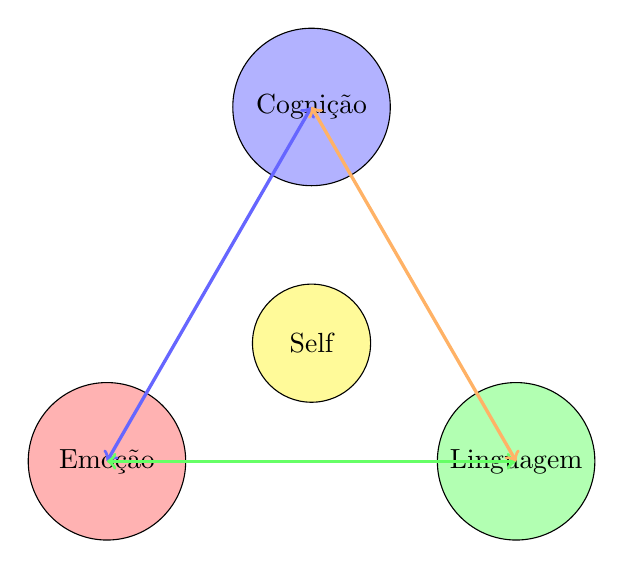
\begin{tikzpicture}[scale=1]
    % Triângulo final
    \coordinate (C) at (90:3);
    \coordinate (E) at (210:3);
    \coordinate (L) at (330:3);

    \node[draw, circle, fill=blue!30, minimum size=2cm] at (C) {Cognição};
    \node[draw, circle, fill=red!30, minimum size=2cm] at (E) {Emoção};
    \node[draw, circle, fill=green!30, minimum size=2cm] at (L) {Linguagem};

    \draw[very thick, <->, blue!60] (C) -- (E);
    \draw[very thick, <->, green!60] (E) -- (L);
    \draw[very thick, <->, orange!60] (L) -- (C);

    \node[draw, circle, fill=yellow!40, minimum size=1.5cm] at (0,0) {Self};
\end{tikzpicture}
\end{center}

\section{A Linguagem como Ferramenta de Diagnóstico e Intervenção}

Exploramos como a linguagem reflete o estado interno do indivíduo, servindo como ferramenta diagnóstica para identificar desordens cognitivas e emocionais. A análise da fala permite ao terapeuta compreender os padrões de pensamento e emoção do paciente, facilitando intervenções direcionadas. A reestruturação verbal atua como instrumento terapêutico, reorganizando o pensamento e promovendo a integração interna.

\section{A Terapia como Ação Comunicativa Emancipatória}

A terapia é apresentada como uma ação comunicativa que visa à promoção da autonomia do paciente. O diálogo autêntico entre terapeuta e paciente, fundamentado na escuta ativa e na empatia, permite a co-construção de significados e a reconstrução da subjetividade. Referências a Carl Rogers, Paulo Freire e Habermas reforçam a importância da comunicação livre de coerção e orientada ao entendimento mútuo.

\section{O Papel da Cultura e das Dinâmicas de Poder}

Reconhecemos que a linguagem e a subjetividade são moldadas pelo contexto sociocultural e pelas dinâmicas de poder. Conforme Foucault, as relações de poder permeiam os discursos, influenciando a forma como os indivíduos se percebem e se expressam. A conscientização dessas influências é essencial para a emancipação e a construção de uma identidade autêntica.

\section{A Evolução Longitudinal da Linguagem}

Acompanhamos como a evolução da linguagem ao longo do tempo reflete a trajetória terapêutica do paciente. A análise longitudinal da fala permite monitorar o progresso, prever crises e ajustar intervenções, promovendo a eficácia do tratamento.

\section{A Busca pela Autenticidade do Ser}

Inspirados por Nietzsche, Kafka, Dostoiévski e Clarice Lispector, exploramos a linguagem como meio de confrontar conflitos internos e buscar a autenticidade. A expressão das emoções mais profundas e a reconstrução das narrativas pessoais são fundamentais para a construção de uma identidade autêntica e autônoma.

\section{Integração Final}

Integrando os conceitos apresentados, propomos que a mente humana é uma totalidade dinâmica constituída pela interdependência entre cognição, emoção e linguagem. A linguagem é o elemento central que permite ao indivíduo nomear suas experiências, organizar seus pensamentos, expressar suas emoções e construir sua identidade.

%% AXIOMAS E TEOREMA
\chapter{Proposta de Axiomas, Postulados e Teorema}

\section{Axiomas}

\begin{axioma}[title=Axioma 1: Interdependência Mental]
Cognição, emoção e linguagem são processos interdependentes que constituem a mente humana. Nenhum desses processos pode ser plenamente compreendido isoladamente dos outros.

\[\forall x, y \in \{C, E, L\}: \frac{\partial x}{\partial y} \neq 0\]
\end{axioma}

\begin{axioma}[title=Axioma 2: Nomeação Existencial]
Nomear é dar existência. A linguagem é o meio pelo qual o indivíduo confere significado às suas experiências e constrói sua realidade interna e externa.

\[\exists(e) \iff \exists N(e)\]

Onde $N(e)$ representa o ato de nomear a experiência $e$.
\end{axioma}

\begin{axioma}[title=Axioma 3: Linguagem Reflexiva]
A linguagem reflete o estado interno do indivíduo, sendo possível inferir o estado cognitivo e emocional a partir da análise da fala.

\[L = f(S_{\text{interno}})\]
\end{axioma}

\begin{axioma}[title=Axioma 4: Transformação Linguística]
A reestruturação da linguagem promove a reorganização interna, permitindo a transformação cognitiva e emocional do indivíduo.

\[\Delta S_{\text{interno}} = g(\Delta L)\]
\end{axioma}

\begin{axioma}[title=Axioma 5: Ação Comunicativa Emancipatória]
A comunicação autêntica e livre de coerção entre indivíduos promove a compreensão mútua, a emancipação e a construção de significados compartilhados.

\[A_{\text{comunicativa}} \Rightarrow \text{Emancipação}\]
\end{axioma}

\begin{axioma}[title=Axioma 6: Influência Sociocultural]
O contexto sociocultural e as dinâmicas de poder influenciam a linguagem e a subjetividade do indivíduo.

\[L = h(P, C, S)\]

Onde $P$ é poder, $C$ é cultura, e $S$ é subjetividade.
\end{axioma}

\section{Postulados}

\begin{postulado}[title=Postulado 1: Terapia Dialógica]
A terapia é um processo dialógico que utiliza a linguagem como instrumento central para promover a integração cognitiva e emocional e a autonomia do paciente.

\[\text{Terapia} = \{\text{Diálogo}(T, P) \mid \text{Objetivo} = \text{Autonomia}\}\]
\end{postulado}

\begin{postulado}[title=Postulado 2: Plasticidade Linguística]
A linguagem é dinâmica e flexível, podendo ser reestruturada para refletir novas compreensões e promover mudanças internas.

\[\forall L_1, \exists L_2: L_1 \rightarrow L_2\]
\end{postulado}

\begin{postulado}[title=Postulado 3: Análise Longitudinal]
A evolução da linguagem ao longo do tempo é um indicador confiável da trajetória terapêutica e do estado mental do indivíduo.

\[\frac{dL}{dt} \propto \frac{dS_{\text{mental}}}{dt}\]
\end{postulado}

\begin{postulado}[title=Postulado 4: Conscientização Sociocultural]
A reflexão crítica sobre as influências socioculturais e de poder na linguagem é essencial para a construção de uma identidade autêntica e autônoma.

\[\text{Reflexão}(L, P, C) \Rightarrow \text{Autenticidade}\]
\end{postulado}

\section{Teorema da Linguagem Transformadora}

\begin{teorema}[title=Teorema da Linguagem Transformadora]
Dado que a linguagem é interdependente com cognição e emoção (Axioma 1) e que a reestruturação da linguagem promove a reorganização interna (Axioma 4), então a intervenção terapêutica que atua sobre a linguagem resulta na transformação cognitiva e emocional do indivíduo, levando à construção de uma identidade autêntica e à promoção da autonomia.

\[\text{Axioma}_1 \land \text{Axioma}_4 \land \text{Postulado}_1 \Rightarrow (\text{Intervenção}_L \Rightarrow \Delta S_{\text{cognitivo-emocional}} \Rightarrow \text{Autonomia})\]
\end{teorema}

\subsection{Demonstração}

\begin{enumerate}
    \item \textbf{Premissa 1} (Axioma 1): Cognição $\leftrightarrow$ Emoção $\leftrightarrow$ Linguagem são interdependentes.
    \item \textbf{Premissa 2} (Axioma 4): $\Delta\text{Linguagem} \Rightarrow \Delta S_{\text{interno}}$
    \item \textbf{Premissa 3} (Postulado 1): Terapia utiliza Linguagem para Integração cognitivo-emocional.
    \item \textbf{Conclusão Intermediária}: De 1, 2 e 3: $\text{Intervenção}_L \Rightarrow \Delta(\text{Cognição} \land \text{Emoção})$
    \item \textbf{Premissa 4} (Axioma 5): $\text{Comunicação}_{\text{autêntica}} \Rightarrow \text{Emancipação}$
    \item \textbf{Conclusão Final}: De 4 e 5: $\therefore \text{Intervenção}_L \Rightarrow \Delta S_{\text{cognitivo-emocional}} \Rightarrow \text{Autonomia}$ \qed
\end{enumerate}

\section{Corolário}

\begin{tcolorbox}[colback=teal!10, colframe=teal!60!black, title=\textsc{Corolário}]
A análise e a reestruturação da linguagem são fundamentais não apenas para a terapia individual, mas também para processos educativos e sociais que visam à emancipação e ao desenvolvimento humano pleno.

\[\text{Análise}_L \land \text{Reestruturação}_L \Rightarrow \{\text{Terapia}, \text{Educação}, \text{Transformação}_{\text{social}}\}\]
\end{tcolorbox}

\section{Considerações Finais}

Este tratado propõe uma compreensão integrada da mente humana, enfatizando o papel central da linguagem na constituição do ser. Ao nomear, o indivíduo confere existência e significado às suas experiências, organizando sua cognição e emoção. A terapia emerge como um espaço privilegiado onde a linguagem é utilizada para promover a autodescoberta, a integração interna e a emancipação.

Reconhecemos a importância de considerar as influências socioculturais e de poder na formação da subjetividade, ressaltando a necessidade de uma reflexão crítica e da promoção da autonomia. Acreditamos que esta compreensão integrada pode contribuir para práticas terapêuticas, educativas e sociais mais efetivas, que valorizem o potencial transformador da linguagem e promovam o desenvolvimento humano em sua plenitude.

\begin{center}
\rule{0.5\textwidth}{0.4pt}
\end{center}

\begin{center}
\textit{``O Tratado Lógico-Afetivo da Linguagem e da Mente Humana: Entre o Nome e o Ser'' busca oferecer uma contribuição significativa para a compreensão da mente humana, integrando diferentes perspectivas teóricas e enfatizando a centralidade da linguagem na constituição do ser. Esperamos que este trabalho inspire reflexões e práticas que valorizem a potência da linguagem como instrumento de transformação pessoal e social.''}
\end{center}

\nextpage
